\section{Comparative study}
\begin{figure}
\centering
  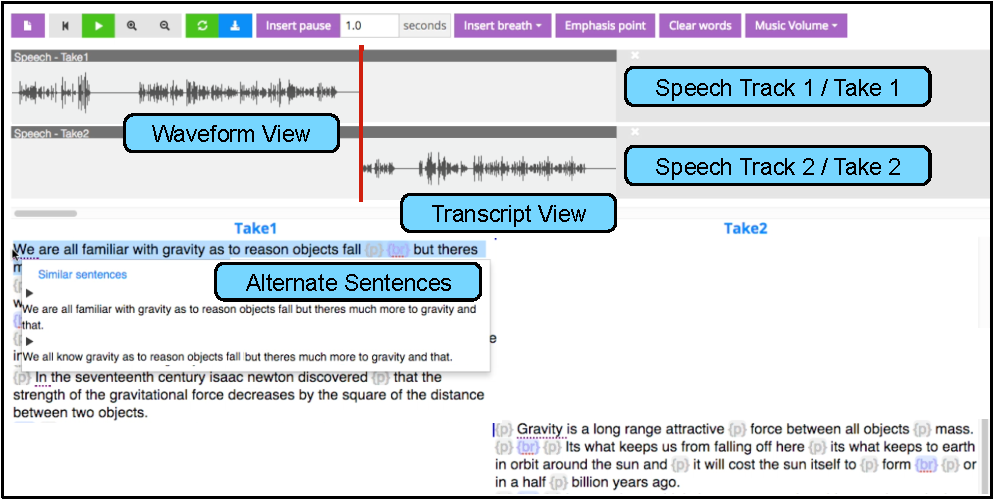
\includegraphics[width=1.0\columnwidth]{figures/interfaceR.pdf}
  \caption{Rubin et al.'s text-based audio editing tool (\textit{Interface-R}). For the purpose of our comparative study, each audio take was loaded as a separate speech track.}~\label{fig:interface-r}
\end{figure}


\begin{table}[t]
\center
\tabcolsep3pt
\begin{tabular}{c|cccccc}
\multicolumn{7}{c}{\textbf{Audio Editing Session}}\\\hline
{User}&\multicolumn{2}{c}{Time spent}& {Total} & {Accept}
&{View}&{Text} \\
{}&\multicolumn{2}{c}{ours \textit{(Rubin)}}&{cuts}&{\textit{ind
/ all}}&{alternate}&{edit}
\\\hline
\textit{A}&\multicolumn{2}{c}{5:58 \textit{(08:10)}}&{3}& {4
/ 3}&{-}&{2}\\
\textit{B}  &\multicolumn{2}{c}{6:40 \textit{(11:10)}}&{3}&{3
/ 4}&{-}&{1}\\
\textit{C}&\multicolumn{2}{c}{9:37 \textit{(11:05)}}&{2}& {7
/ -}&{1}&{7}\\
\textit{D}&\multicolumn{2}{c}{7:25 \textit{(09:10)}}&{6}& {10
/ 1}&{3}&{-}
\\\hline
\end{tabular} 
\label{tab:editing}
\caption{Four participants created audio
recordings from two pre-recorded takes, using our interface and
Rubin et al.'s interface. Usage statistics pertain to our interface.
Accept \textit{ind / all} are number of segments accepted from
the individual transcript view and the \textit{all} tab view
respectively.}
\end{table} 

\VREV{One of the main tasks in creating audio recordings is cutting and merging multiple audio takes. There are many existing software that specifically assist this task (see Related Work). We conducted a pilot study to explore whether our master-script view facilitates audio editing compared to a state-of-the-art speech transcript-based editing interface }\cite{rubin2013content}. 

\VREV{Similar to \textit{Voice Script}, Rubin et al.'s interface (shown in} Figure~\ref{fig:interface-r}, \VREV{and referred to as
\textit{Interface-R} hereafter) also uses time-aligned transcripts to support text-based editing. In both systems, users
can edit the transcript like a text document using operations
such as copy-and-paste, insert, or delete, and the edits are propagated
to the audio. Both systems also detect alternate takes of the
same sentence and groups them together so that users can easily compare and select between them.
However, unlike \textit{Voice Script} , Interface-R does have a master-script that integrates multiple audio recordings with a script. In fact, Interface-R does not explicitly handle multiple recordings. To simulate
multiple takes, we took advantage of their multiple speech tracks,
so that each take appeared in a separate speech track (i.e., separate columns).}

We recruited 4 participants, none of whom had
prior experience using text-based audio editing systems. We gave them
a script with bullet points outlining a mini lecture on a technical
subject (e.g. \textit{gravity} and \textit{dark matter}) and
two audio takes roughly corresponding to the script. \VREV{In \textit{Voice Script}, the script was contained in the initial master-script. On the other hand, since Interface-R does not have a notion of
a script separate from the transcripts, we gave users a hard copy
of script.} The task
was to cut and merge the two pre-recorded takes to produce a recording that
contained all the contents listed in the script and only those
contents. The two takes were similar, but each take had some
missing content and some extra
content. The participants had to choose parts from each take
and combine them to get the final result. We encouraged the users
to focus on having the complete content rather than on the details
of the audio quality (e.g. tempo, diction, flow of speech etc.).


Each participant completed the task twice, once on each interface using different scripts.
The subject of the lecture and the order of the interface were
counter-balanced. We examined the time users spent to complete the task, the number/type of functions they used, and the quality of the
final recording. After each task, participants gave written
qualitative feedback about their experience. In total, each
session lasted about 1 hour. \VREV{Below are our key findings.} 
   
\VREV{\textbf{Users completed the task faster using Voice Script.} All participants completed the task faster using our interface (average 7.4  \textit{vs} 9.9 min), and also preferred it to Interface-R. The difference may be accounted for by the different workflow that each interface affords. In Interface-R, users effectively started with both recordings in the final track. Then, they applied copy-and-paste to cut and merge the two takes, and deletion to remove redundant or superfluous content. In contrast, in \textit{Voice Script}, users effectively started with an empty final track. Then, using the \textit{compare-view} they \textit{accepted} parts that matched the script from either of the takes. Although copy-and-paste and deletion  were also available in \textit{Voice Script} these operations were  used sparsely, for example to delete a mistakenly accepted segment, to delete individual words, or to change the ordering of accepted segments (Table 1)} .  %Each of the four participants preferred \systemname\ over Interface-R %for the given task, and noted they would use
% our interface to edit audio recordings. Every participant also
% completed the task faster using our interface (7.4 $vs$ 9.9 min Interface-R). 
% Table 2 summarizes the participants' usage of our interface. Again users had different preferences for the individual transcript view and the \textit{all-tab} view. User B wrote,  \textit{``individual tabs were helpful after using the all-tab to make sure I hadn't missed content''} whereas user D \textit{``liked the individual tabs better since I wanted to view the original take as is.''} For this task, participants did not have to insert new content, but they used text editing operations to move content (e.g. copy \& paste)\ or delete portions of accepted segments from the final track.   

\VREV{\textbf{The master-script facilitates merging by integrating the script and the recordings.} Users appreciated having the master-script view. First, the master-script served to integrate the script outline and the recordings into a single comprehensive document. To quote from one user, \textit{``The master view integrated the two takes into an almost seamless whole that I just had to edit, as opposed to presenting two separate draft from which I had to generate a third and final story.''}  Secondly, the master-script helped users keep track of the status of the final track compared to the planned script. One user noted that \textit{``The outline [in the master-script] made it easier to find what I had accepted to the final track and what was still missing, instead of making notes on the paper outline and going back-and-forth between it and the recordings.'' } } 

\VREV{\textbf{The alignment between script and transcripts facilitates merging.}  All 4 participants mentioned the \textit{align} function in the \textit{compare-view} as the most helpful feature in \textit{Voice Script}. First, as one user noted, the segmentation in \textit{``the alignment view made editing much faster by visually breaking the script and the transcript into corresponding parts. I found I had to read much less.''} Also users found it \textit{``easier to click than to copy and paste''} in order to merge portions of recordings into the final track.    
}
